\subsubsection{Uroflowmetry}


\begin{enumerate}
    \item 3D print or manufacture the supporting parts using the STL files
    \begin{figure}[h]
        \centering
        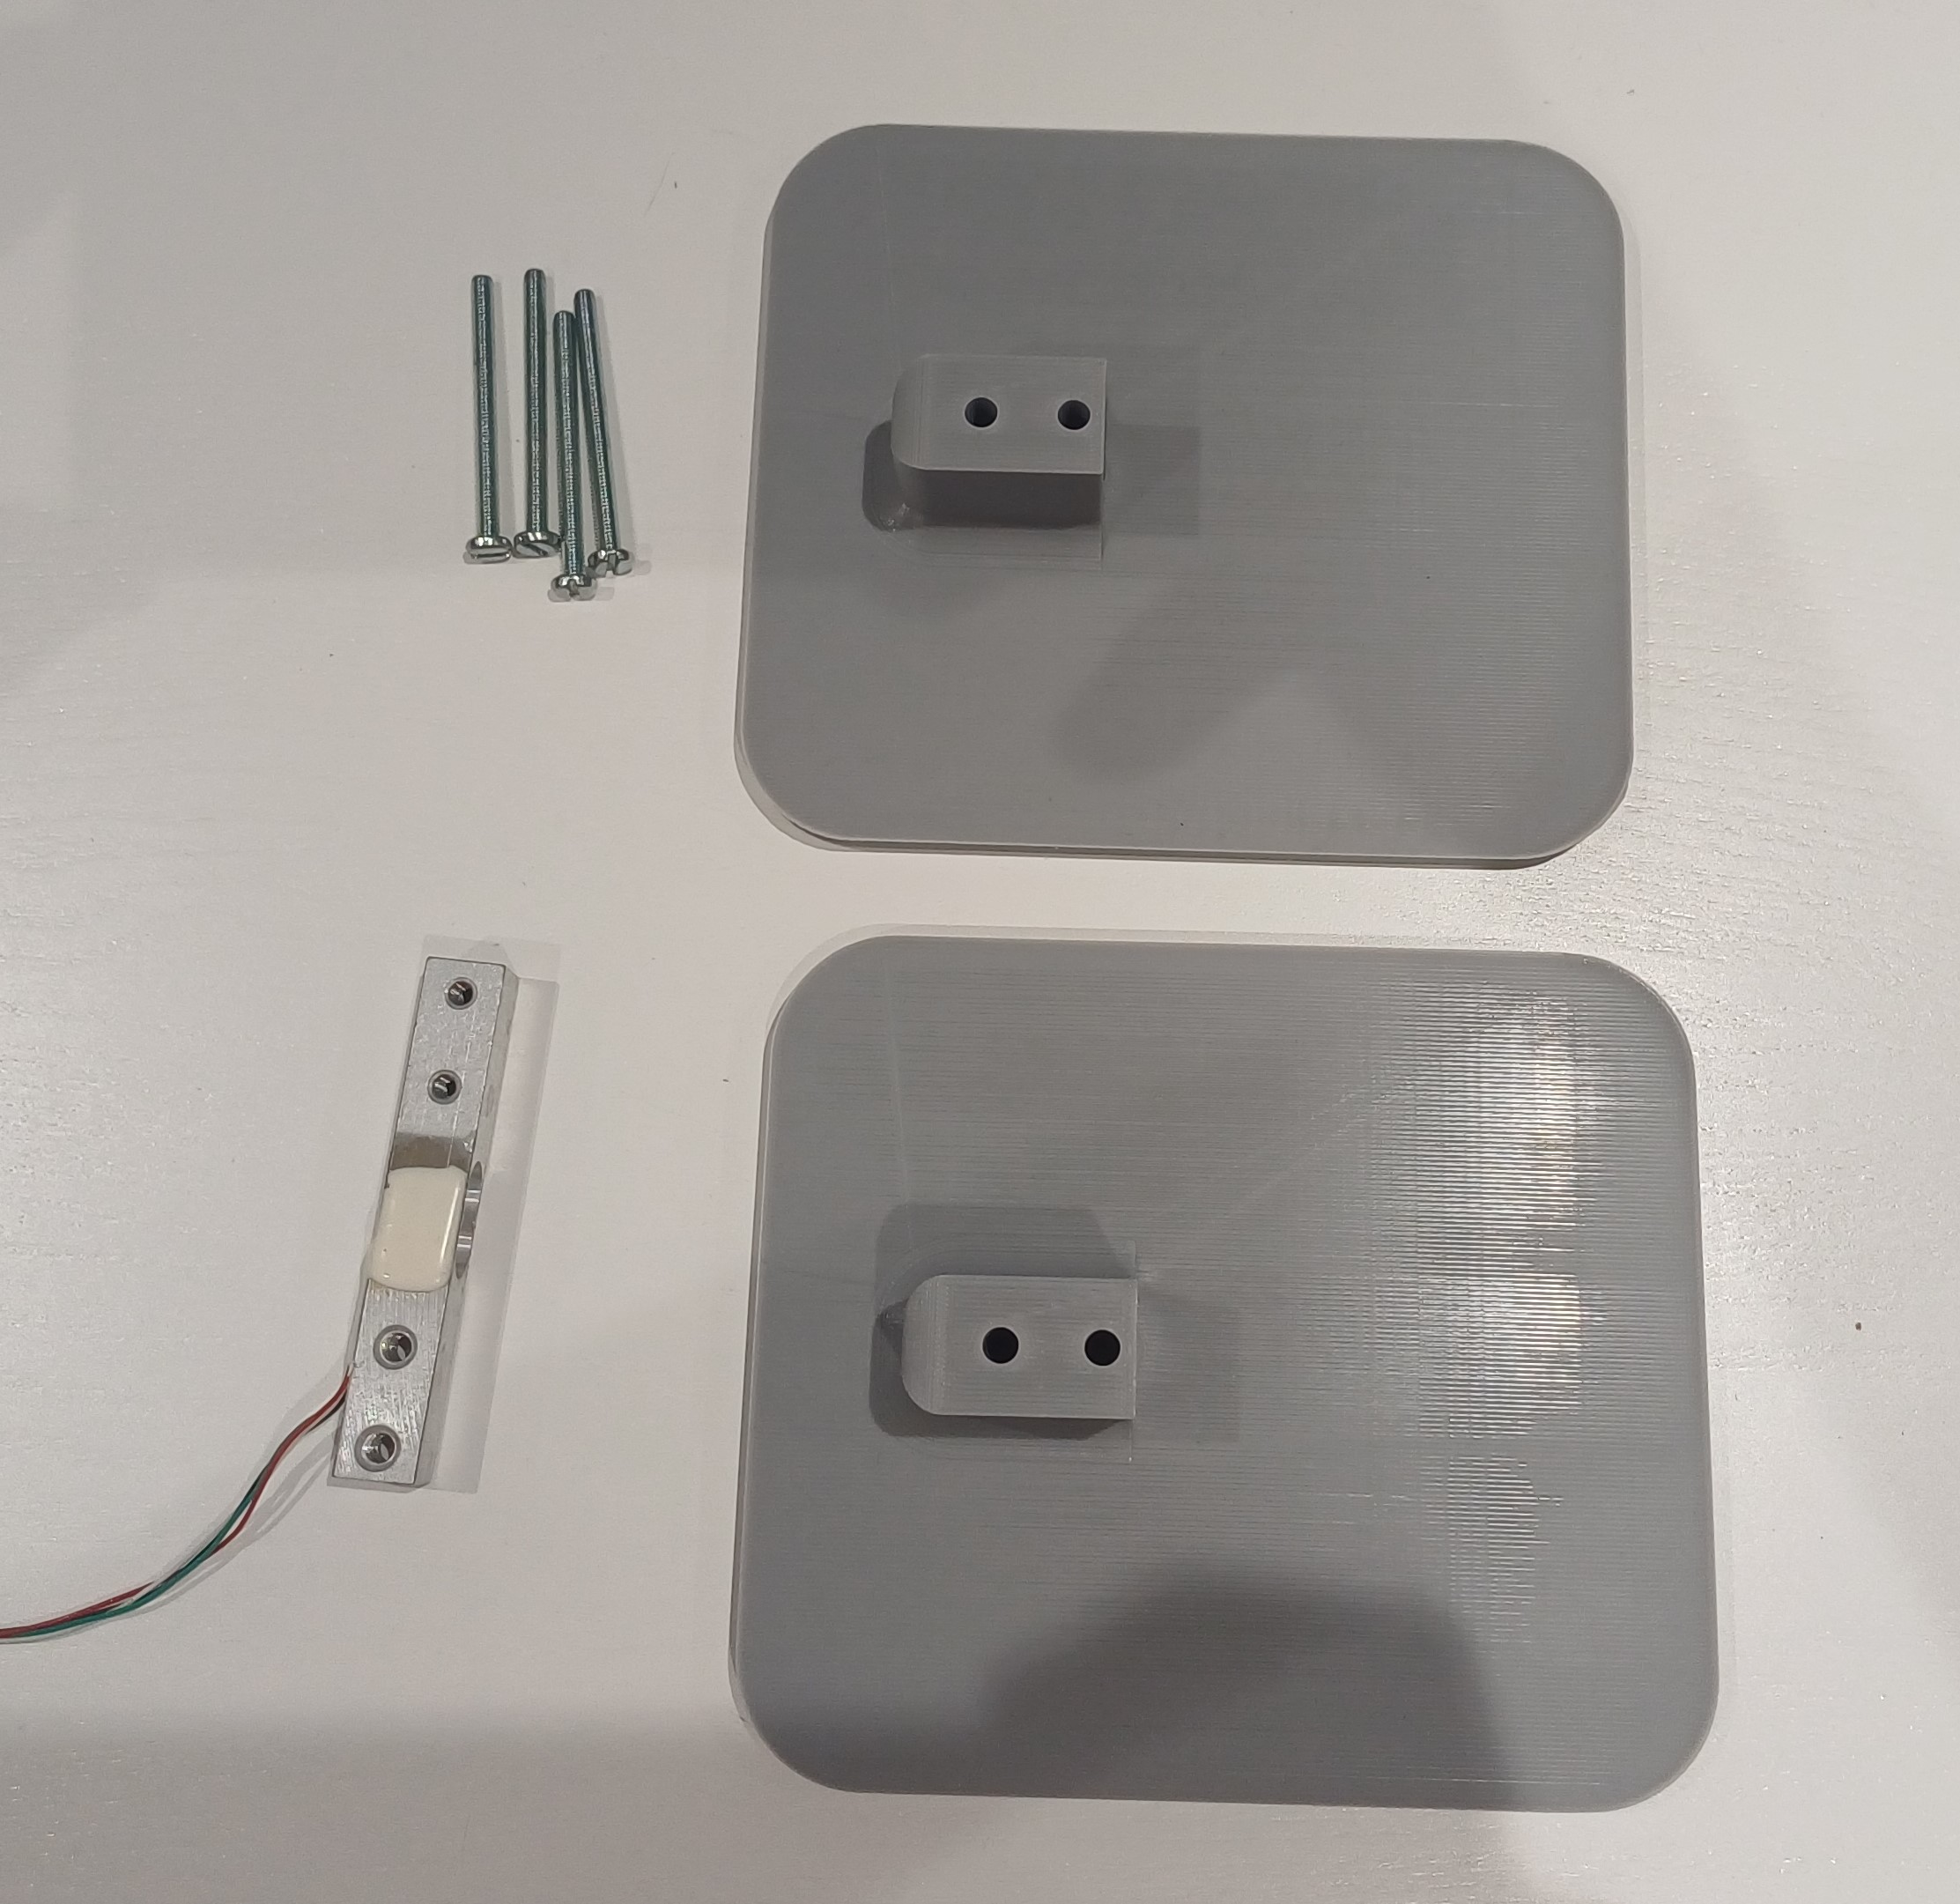
\includegraphics[width=0.7\textwidth]{Figures/Manufacture/Uroflowmetry/uf_required_parts.jpg}
        \label{fig:ufrequiredparts}
      \end{figure}
    \item Connect the 2m 4 core wire to the 4 wires attached to the loadcell (Note the order of the wires attached)
    \item Solder the male 4 pin DIN connector to the other end of the 
    \item Screw the loadcell into the first baseplate
    \begin{figure}[h]
        \centering
        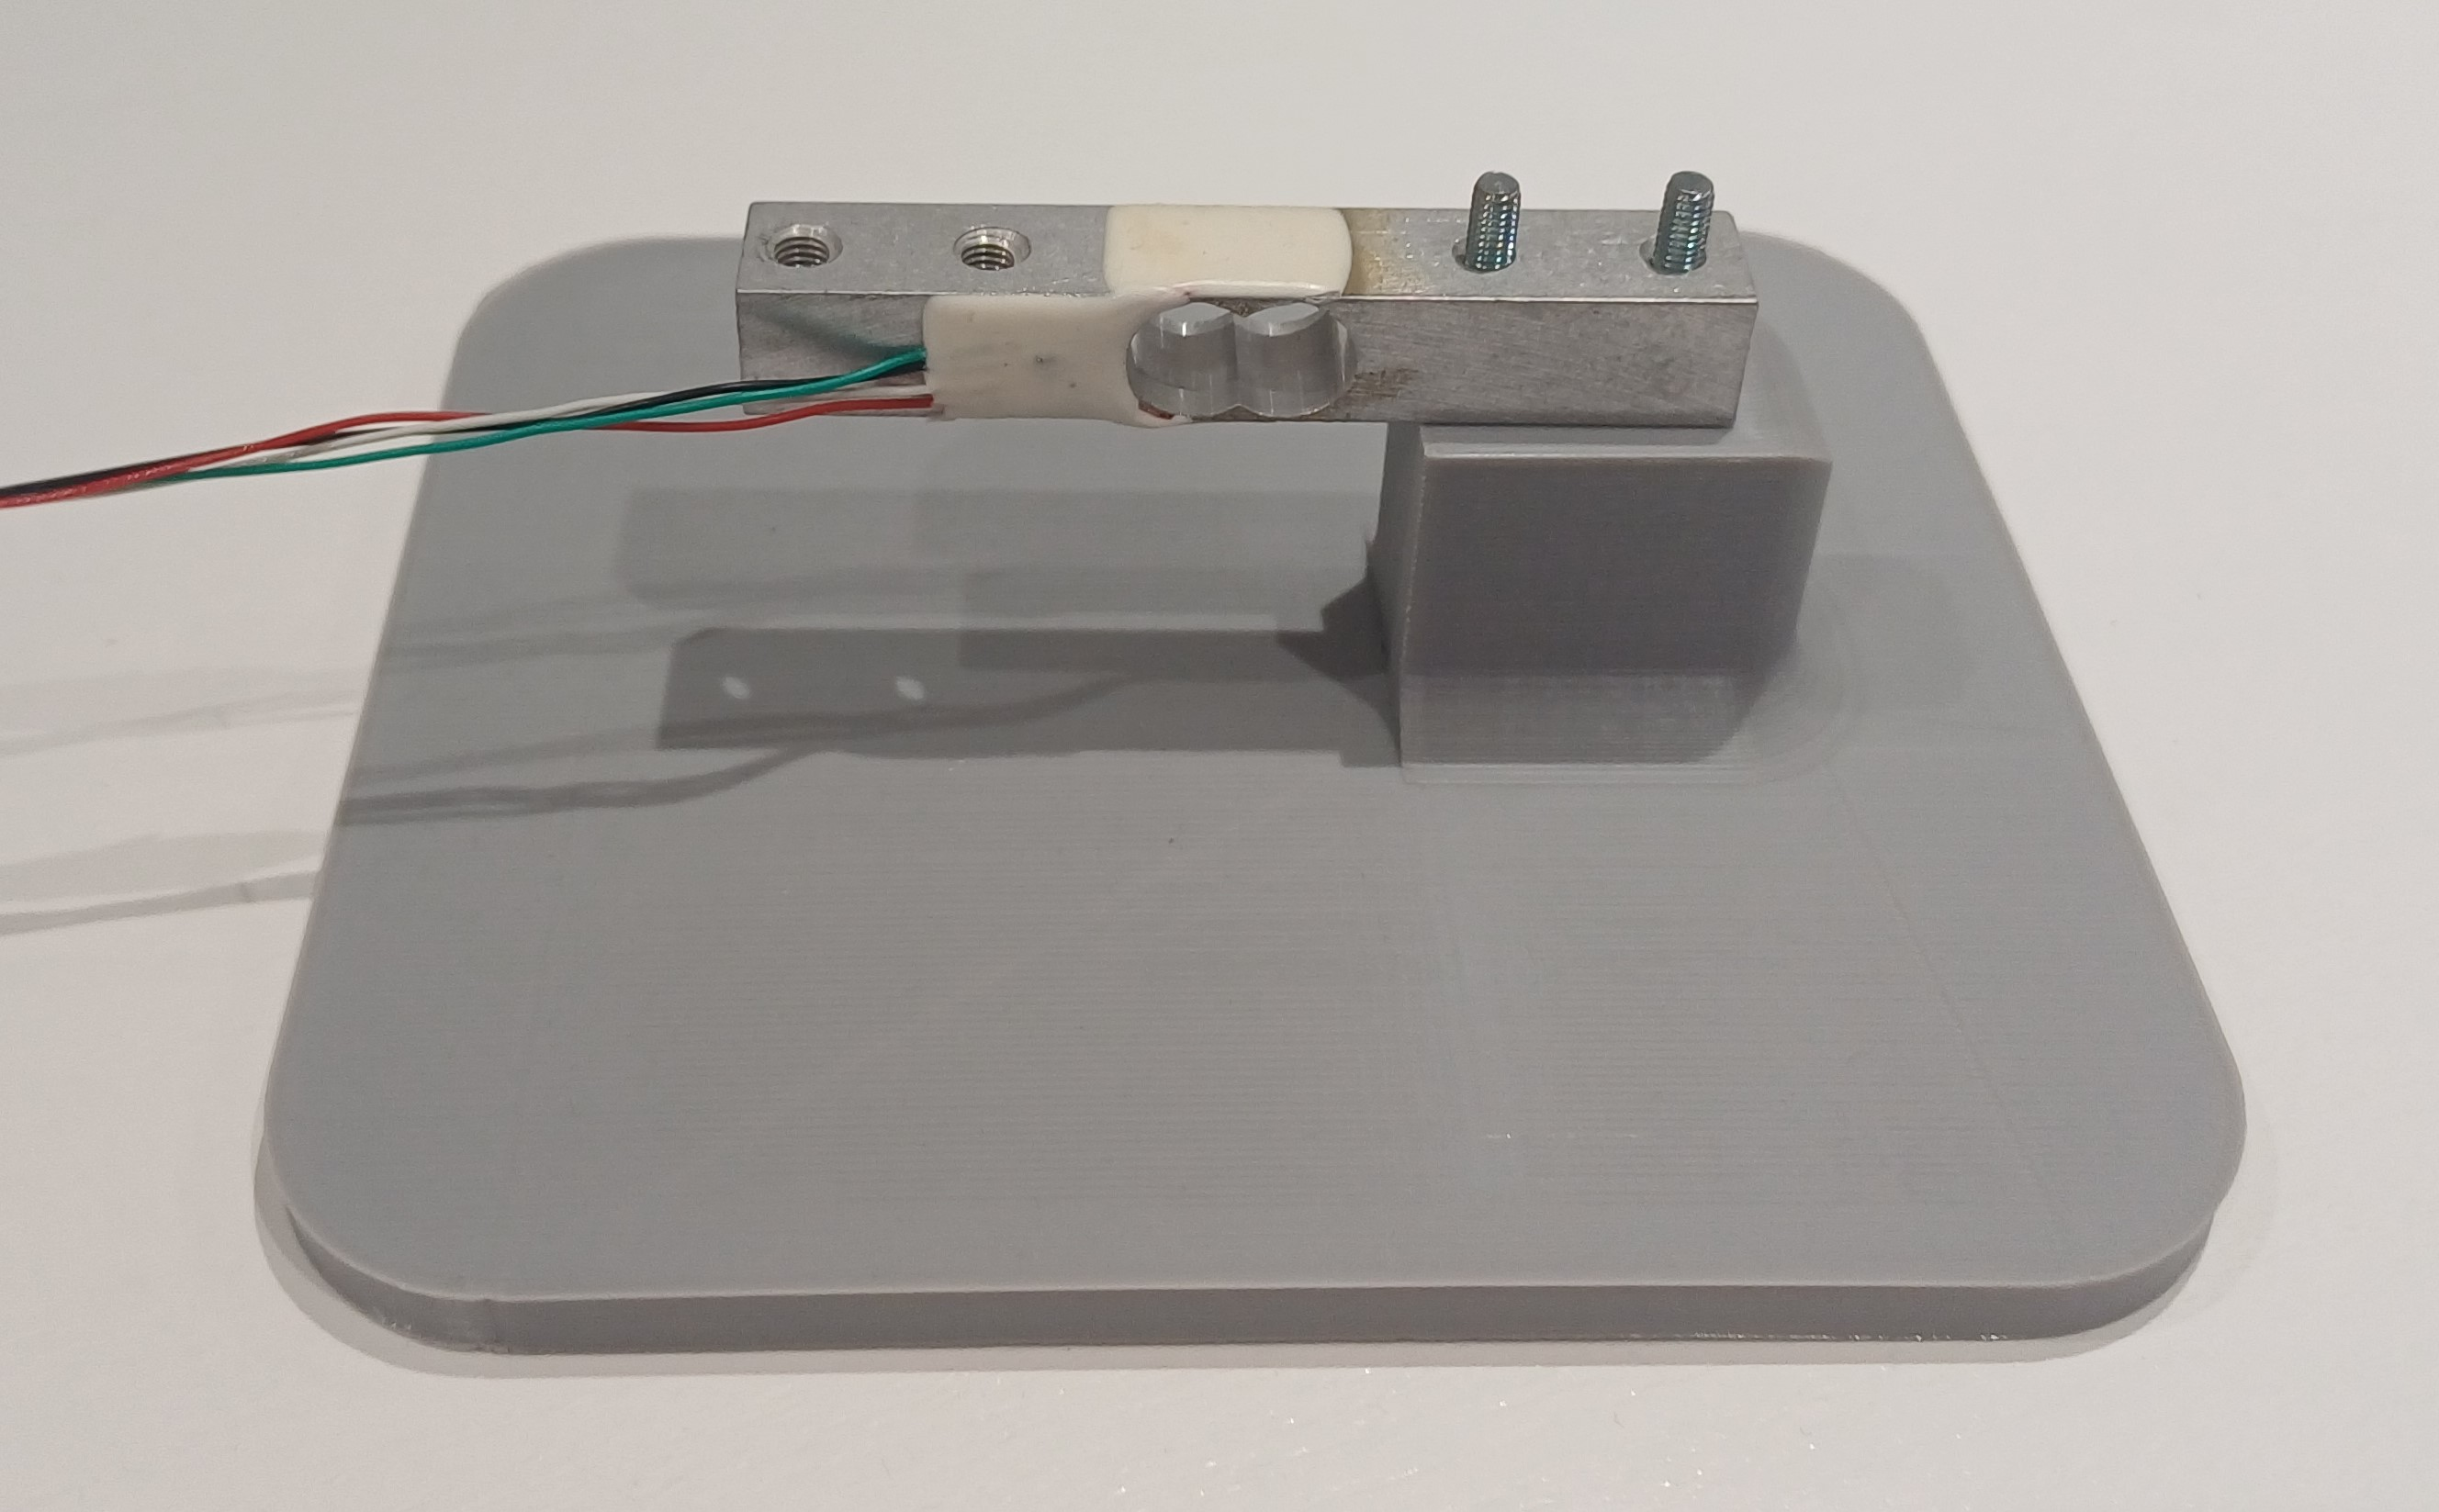
\includegraphics[width=0.7\textwidth]{Figures/Manufacture/Uroflowmetry/uf_screw_first_baseplate.jpg}
        \label{fig:ufscrewfirstbaseplate}
      \end{figure}
    \item Screw the second base plate onto the loadcell
    \begin{figure}[h]
        \centering
        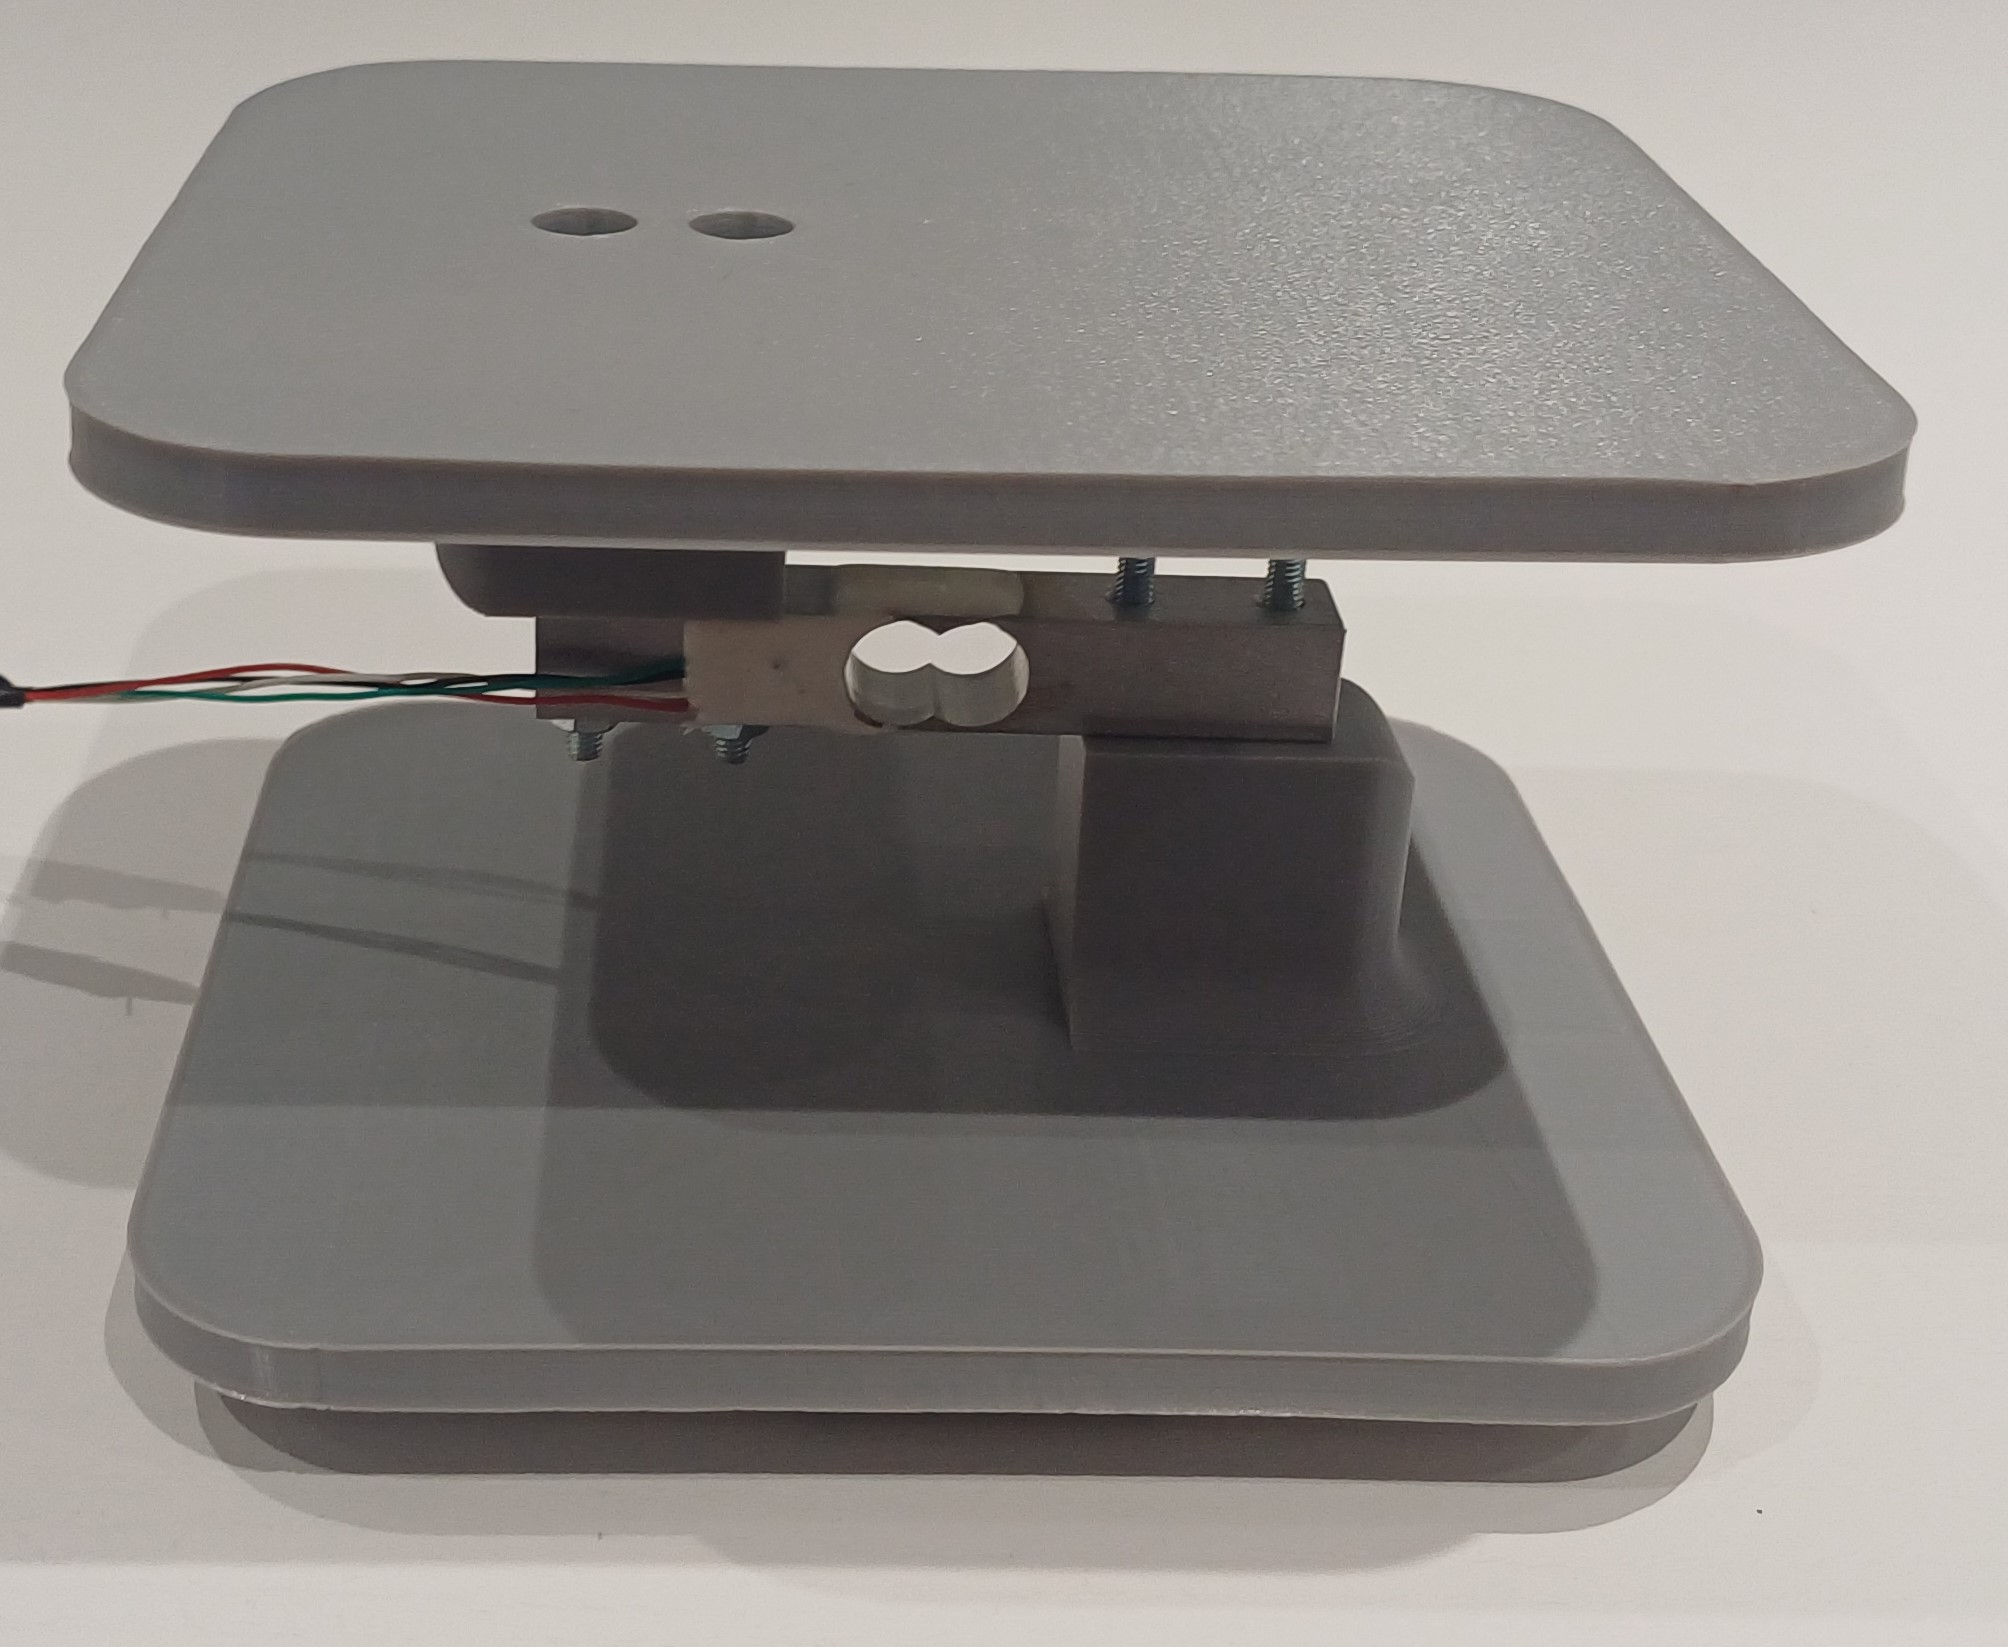
\includegraphics[width=0.7\textwidth]{Figures/Manufacture/Uroflowmetry/uf_screw_second_baseplate.jpg}
        \label{fig:ufscrewfirstbaseplate}
      \end{figure}
  \end{enumerate}
  